\NeedsTeXFormat{LaTeX2e}
\documentclass[11pt]{article}
\usepackage{url}
\usepackage{amsmath}
\usepackage{amsthm}
\usepackage{amssymb}
\usepackage{mathpartir}
\usepackage{graphicx}
\usepackage{comment}


\newcommand{\deftech}[1]{\textbf{#1}}
\newcommand\mrel{\mathop{\mathbf{r}}}
\newcommand\morel{\mathop{\mathbf{r}'}}
\newcommand\menv{\rho}
\newcommand\mval{v}
\newcommand\mans{a}
\newcommand\mint{i}
\newcommand\moint{j}
\newcommand\mbool{b}

\newcommand\plug[2]{#1[#2]}

\newcommand\merr{r}

\newcommand\mctx{\mathcal{C}}
\newcommand\mectx{\mathcal{E}}
\newtheorem{theorem}{Theorem}
\newcommand\Err{\mathit{Err}}
\newcommand\Plus{\mathit{Plus}}
\newcommand\Mult{\mathit{Mult}}
\newcommand\Succ{\mathit{Succ}}
\newcommand\Pred{\mathit{Pred}}
\newcommand\Eq{\mathit{Eq}}
\newcommand\True{\mathit{True}}
\newcommand\False{\mathit{False}}
\newcommand\If{\mathit{If}}
\newcommand\Div{\mathit{Div}}

\newcommand\reduce{\mathop{\mathbf{b}}}

\newcommand\areducename{\mathbf{a}}
\newcommand\areduce[2]{#1\;\areducename\;#2}

\newcommand\step{\rightarrow_\mathbf{b}}
\newcommand\multistep{\rightarrow^\star_\mathbf{b}}

\newcommand\astdstep{\longmapsto_{\reduce}}
\newcommand\astdmultistep{\longmapsto^\star_{\reduce}}

\newcommand\breducename{\mathbf{b}}
\newcommand\errreducename{\mathbf{err}}
\newcommand\propreducename{\mathbf{prop}}
\newcommand\bvreducename{\mathbf{bv}}
\newcommand\bstepname{\rightarrow_{\breducename}}
\newcommand\bmultistepname{\rightarrow^\star_{\breducename}}

\newcommand\bmultistep[3]{#1\vdash #2\;\bmultistepname\;#3}
\newcommand\bstdstep[3]{#1\vdash #2\;{\longmapsto_{\breducename}}\;#3}
\newcommand\bstdmultistep[3]{#1\vdash #2\;{\longmapsto^\star_{\breducename}}\;#3}

\newcommand\breduce[3]{#1 \vdash {#2}\;\breducename\; {#3}}
\newcommand\errreduce[3]{#1 \vdash {#2}\;\errreducename\; {#3}}
\newcommand\propreduce[3]{#1 \vdash {#2}\;\propreducename\; {#3}}
\newcommand\bvreduce[3]{#1 \vdash {#2}\;\bvreducename\; {#3}}
\newcommand\bstep[3]{#1 \vdash {#2}\;\rightarrow_{\breducename}\; {#3}}
\newcommand\bclosedstep[2]{{#1}\;\rightarrow_{\breducename}\; {#2}}

\newcommand\laxparstep{\rightrightarrows_\mathbf{a}}
\newcommand\maxparstep{\rightrightarrows'_\mathbf{a}}


\newcommand{\xdown}[1]{X_{#1 \downarrow}}
\newcommand{\xup}[1]{X_{#1 \uparrow}}
\newcommand{\xdownk}[2]{X_{#1 \downarrow #2}}
\newcommand{\xupk}[2]{X_{#1 \uparrow #2}}
\newcommand{\xblock}[1]{[x_{#1 1}, x_{#1 2} , \dots, x_{#1 \frac{1}{c}}]^{\top}}
\newcommand{\conpr}[2]{Pr[#1\,|\,#2]}
\newcommand{\priv}{{\bf priv}(X)}
\newcommand{\alt}[1]{{\bf alt}(X_{#1})}
\newcommand{\xbot}[1]{x_{#1 \frac{1}{c}}}
\newcommand{\cwp}[1]{(\epsilon, \delta, \Delta_{#1}, \Gamma)}


\newcommand\Arith{\mathcal{A}}
\newcommand\Barith{\mathcal{B}}

\newcommand\Var{\mathit{Var}}

\newcommand{\mvar}{x}
\newcommand\s[1]{\mathit{#1}}

\title{Composition Theorem for streaming CW-pricacy}
\date{}
\begin{document}
\maketitle

\section{Characterize Privacy as Regions}
In this section, we show how to characterize Differential Privacy (DP) and CW-Privacy (CW-P) in terms of convex regions, and how to compute the $(\epsilon, \delta)$ values for each mechanism in terms of tangent lines of such convex regions. We focus on the context of finite discrete states for the simplicity of analysis.
\subsection{Case of DP}
Let ${\cal X} $ be the set of all databases. Let ${\cal Y}$ be the set of all out comes of mechanism $M$. $M$ is a probability measure from $\cal X$ to $\cal Y$. For simplicity of analysis, assume $|{\cal X}| =n $ and $|{\cal Y}|=m$. Then, $M$ corresponds to an $n \times m$ Markov matrix ${M} =[M(x_{1}), \dots , M(x_{n})]^{\top}$.


Now, it is easy to see the following is an equivalent definition of DP.
\begin{theorem}
For any $\epsilon \geq 0$ and $\delta \in [0, 1]$, a mechanism $M$ is $(\epsilon, \delta)$-differentially private if and only if the following conditions are satisfied for all pairs of neighboring databases $x$ and $x'$, and all region $S \subseteq {\cal Y}$:
\[
Pr[M(x) \in S]+e^{\epsilon}Pr[M(x') \in \bar{S}] \geq 1-\delta , \quad and
\]
\[
e^{\epsilon}Pr[M(x) \in S]+Pr[M(x') \in \bar{S}]  \geq 1-\delta .
\]
\end{theorem}
This gives a graphical representation (region) of DP:
\[
R(\epsilon, \delta) = \{(p_{x},p_{y}) \,|\, p_{x}+e^{\epsilon}p_{y} \geq1 - \delta,  e^{\epsilon}p_{x}+p_{y} \geq 1 - \delta\} .
\]
For any two databases $x$ and $x'$, define
\[
R(M, x, x') = convex \{(Pr[M(x) \in S], Pr[M(x') \in \bar{S}]) \,|\, \text{for all }S \subseteq {\cal Y} \}
\]
$R(M,x,x')$ has the following equivalent form.
\[
R(M,x,x') = \{ (M(x) \cdot {\bf \alpha}, M(x') \cdot {\bf \beta}) \,|\, 0 \leq \alpha_{i}, \beta_{i} \leq 1, \, {\bf \alpha} +{\bf \beta} = {\bf 1^{m}} \},
\] 
where $\cdot$ denote the dot production of vectors.
\begin{definition}
For any mechanism $M$, we define its privacy region $R(M) = \bigcup_{(x , x')} R(M, x, x') $, where $(x,x')$ is a pair of neighboring databases.
\end{definition}
Immediately, it should not hard to see the following theorem.
\begin{theorem}
 $M$ is $(\epsilon, \delta)$-differentially private iff $R(M) \subseteq R(\epsilon, \delta) $.
 \end{theorem}
\begin{figure}[th]
\centering
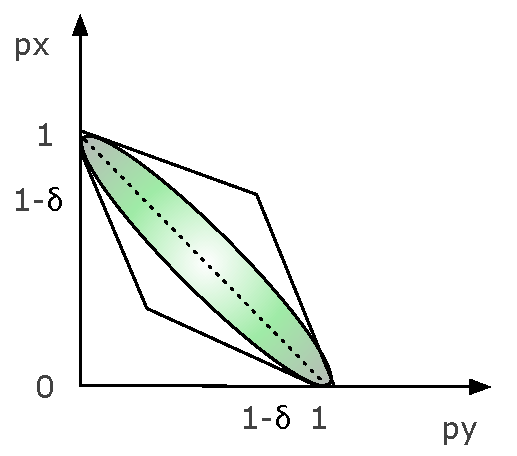
\includegraphics[width=2.5in]{fig/privacyregion.pdf}
\caption{\label{privacy_region} Every tangent line of the privacy region forms a pair of $(\epsilon, \delta)$. }
\end{figure}
As it is shown in Figure~\ref{privacy_region}, every tangent line of the privacy region corresponds to a pair of $(\epsilon, \delta)$. In general, the privacy region $R(M, x, x')$ of any mechanism $M$ can be represented by the intersections of all such regions $\{R(\epsilon_{i}, \delta_{i})\}$, which is completely described by the set of slopes and shifts $\{(\epsilon_{i}, \delta_{i})\}$.
\begin{enumerate}
\item For the set slopes, let ${\cal E} = \{0 \leq \epsilon_{i} < \infty \,|\, Pr[M(x)=y] = e^{\epsilon_{i}}Pr[M(x')=y] \text{ for some $y \in {\cal Y}$} \}$
\item For each $\epsilon_{i}$,  $\delta_{i} = \max_{S \subseteq {\cal Y}} \{ \Sigma_{y \in S}Pr[M(x)=y] - e^{\epsilon_{i}}\Sigma_{y \in S}Pr[M(x)=y]\}$
\end{enumerate}
\subsection{Case of CW-P}
In the case of CW-P, we use $X$ to denote a database variable that follows some distribution $D$. Let the pmf of $D$ be $f_{D} =[{f_{x_{1}} , \dots, f_{x_{n}}}]$. Let $alt(X)$ denote a scrubbed version of $X$. Assume $alt(X)$ follows some distribution $D'$ with pmf $f'_{D}$.

It is easy to see that CW-P has the following equivalent definition.
\begin{theorem}
For any $\epsilon \geq 0$ and $\delta \in [0, 1]$, a mechanism $M$ is $(\epsilon, \delta,\Delta, \Gamma)$-differentially private if and only if the following conditions are satisfied for all distributions on $D$ on $(X, Z)$, all $(priv, alt) \in \Gamma$ pairs, and all region $S \subseteq {\cal Y}$:
\[
Pr[M(X) \in S \,|\, priv(X), Z]+e^{\epsilon}Pr[M(alt(X)) \in \bar{S}\,|\, priv(X), Z] \geq 1-\delta , \quad and
\]
\[
e^{\epsilon}Pr[M(X) \in S\,|\, priv(X), Z]+Pr[M(alt(X)) \in \bar{S}\,|\, priv(X), Z]  \geq 1-\delta ,
\]
where $M(X) = f_{D}M$ and $M(alt(X))=f'_{D}M$.
\end{theorem}
Notice mechanism $M' = [f_{D}M, f'_{D}M]^{\top}$ can be seen as a DP version of $M$. Hence, CW-P also has form of privacy regions, and everything else described above follows.
\section{Composition Theorem of CW-P in the streaming setting}
\begin{figure}[th]
\centering
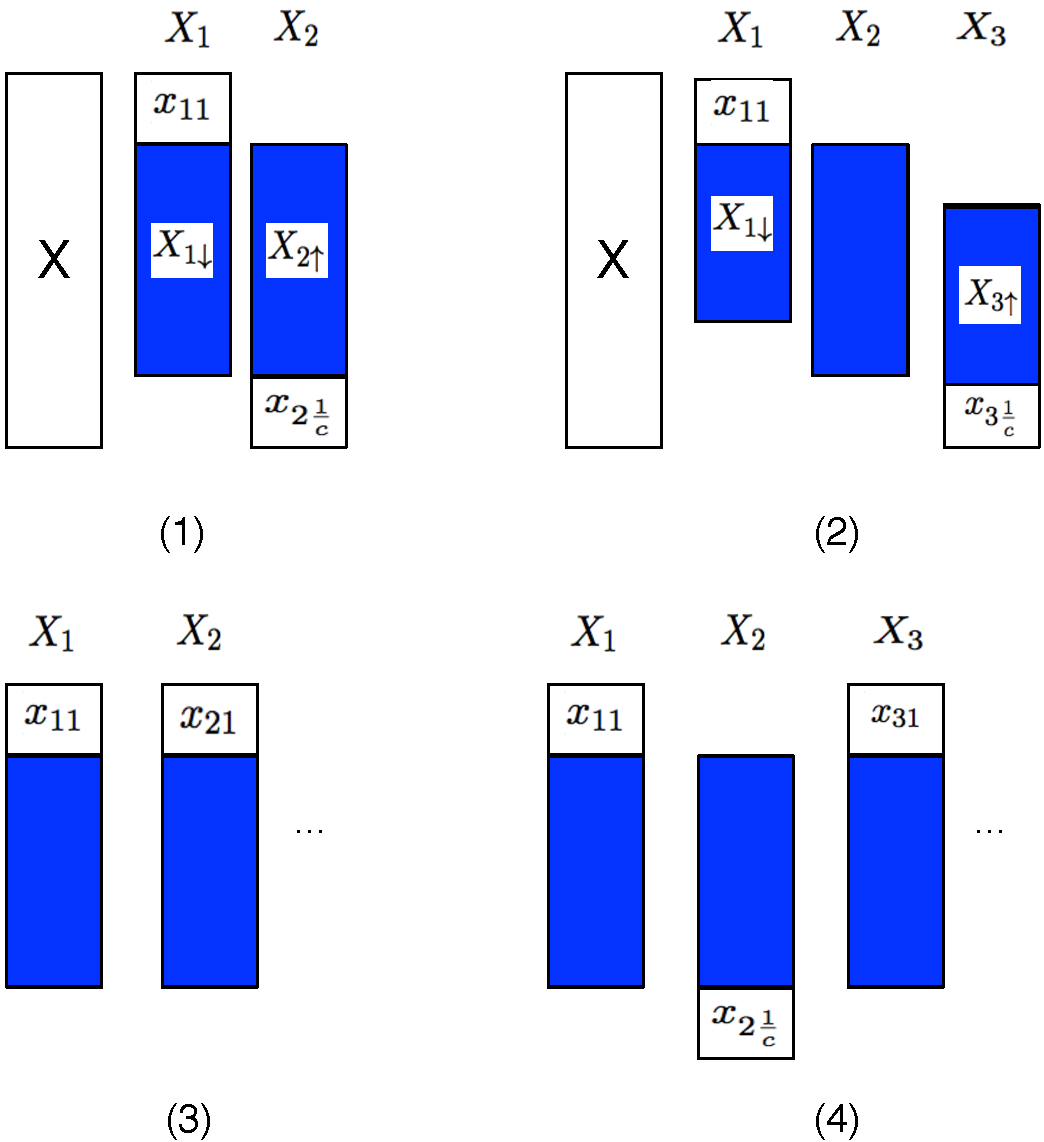
\includegraphics[width=4.8in]{fig/stream_database1.pdf}
\caption{\label{stream_db1} Blocks in blue are shared by more than one databases. Blocks in white are owned by only one database. (1) Composition of $F(X_{1})$ and $F(X_{2})$. It has ``good" independence since each $X_{i}$ owns one block. (2) Composition of queries on three streaming databases. Cannot leverage ``good" independence, because each block in $X_{2}$ is shared by two databases. (3) Composition of queries in the standard DP case. The blue blocks refer to the query while the white blocks refer to the independent noise. (4) It works as long as each streaming database owns one block of ``private" block.}
\end{figure}
{\bf Problem setting} \\
Let $X$ be a database in the streaming setting. Let $X_{i}$ represent the portion of $X$ that is currently held at time step $i$. We assume that at each time step, a fraction of $c$ of the database is replaced. We assume the oldest rows are always the ones replaced, and that $X$ has row drown i.i.d. from some distribution $D$. Let $n$ be the size of each $X_{i}$. This means that the first $n$ rows of $X$ constitute $X_{1}$, rows $cn+1$ through $cn+n$ constitute $X_{2}$, and so forth. $X$ has size $n+cn(t-1)$, where $t$ is the total number of time steps being considered. $1/c$ is the total number of time steps a given row will be present for. See (1) and (2) in Figure~\ref{stream_db1}. 
\\
\\
{\bf Notations }\\
For each $X_i$ of size $n$, we represent it by $1/c$ blocks (each has $cn$ rows). Namely, let $X_{i}=\xblock{i}$, where $x_{ij}$ denote the $j$th block in $X_{i}$. Let $\xdown{i} = [x_{i 2} , \dots, x_{i \frac{1}{c}}]^{\top}$ and $\xup{i} = [x_{i 1}, x_{i2} , \dots, x_{i (\frac{1}{c}-1)}]^{\top}$. Namely, $\xdown{i}$ represent the bottom $(1/c -1)$ blocks of $X_{i}$ while $\xup{i}$ represent the top $(1/c-1)$ blocks of $X_{i}$.

Consider a mechanism $M: \, {\cal X} \rightarrow {\cal Y}$ on each $X_{i}$. We assume $|{\cal X}| =n$ and $|{\cal Y}|=m$ for the simplicity of analysis. Let each $X_{i}$ follows some distribution $D$ with pmf $f_{D}$. Let each $alt(X_{i})$ follows some distribution $D'$ with pmf $f'_{D}$.
\\
\\
{\bf Assumptions}
\begin{enumerate}
\item $M$'s auxiliary information consists of {\bf the last $(1-c)n$ rows} of the database $X_{i}$, i.e., $\xdown{i}$ is given. We denote the pmf of $X_{i}$ conditioned on $\xdown{i} =z$ as ${f_{D}}_{|\xdown{i} = z}$. We denote the pmf of $alt(X_{i})$ conditioned on $\xdown{i} =z$ as ${f'_{D}}_{|\xdown{i} = z}$. For all $z$ and all $x \in {\cal X}$, we assume $$\frac{{f_{D}}_{|\xdown{i} = z} (x)}{{f'_{D}}_{|\xdown{i} = z}(x)} \leq e^{\gamma},$$ where $\gamma>0$ is a small constant.
\item According to section 1, $M$ can be characterized as a convex region. It should have a set of $(\epsilon_{j}, \delta_{j})$ values that are computable by its tangent lines. We assume that there is a subset ${\cal W} \subseteq {\cal Y}$ such that (we ignore the $priv(X_{i})$ in the expression)
\begin{enumerate}
\item $\forall y \in {\cal W},\, \forall z: \conpr{M(X_{i})=y}{\xdown{i}=z} \neq 0 \text{ , }\conpr{M(alt(X_{i}))=y}{\xdown{i}=z} \neq 0$ ;
\item $\forall y \in {\cal Y-W},\, \forall z: \conpr{M(X_{i})=y}{\xdown{i}=z} = 0 \text{ , }\conpr{M(alt(X_{i}))=y}{\xdown{i}=z} = 0$ .
\end{enumerate}
For each $y_{j} \in {\cal W}$ and for all $z$, let 
\begin{equation}
 e^{\epsilon_{j|z}} = \frac{\conpr{M(X_{i})=y_{j}}{\xdown{i}=z} }{\conpr{M(alt(X_{i}))=y_{j}}{\xdown{i}=z} } \geq  1.
\end{equation}
For each $\epsilon_{j|z}$, it has a corresponding $\delta_{j|z}$ such that
\begin{equation}
\delta_{j|z} =\max_{S \subseteq {\cal W}} \{ \Sigma_{y \in S}\conpr{M(X_{i})=y_{j}}{\xdown{i}=z} - e^{\epsilon_{i}}\Sigma_{y \in S}\conpr{M(alt(X_{i}))=y_{j}}{\xdown{i}=z}\} 
\end{equation} 
For each $j$, let $\min_{z} \{\epsilon_{j|z} \}= \epsilon_{j|min}$ and $\max_{z} \{\epsilon_{j|z} \}= \epsilon_{j|max}$. Obviously, the minimal shift $\delta_{j|min}=\min_{z} \{\delta_{j|z}\} $ is computed by $\epsilon_{j|max}$. The maximal shift $\delta_{j|max}=\max_{z} \{\delta_{j|z}\} $ is computed by $\epsilon_{j|min}$. Let $\epsilon_{max} = \max_{j} \{\epsilon_{j|max}\}$, which corresponds to $\delta_{min} = \min_{j} \{\delta_{j|min}\}$.

Let ${\cal E} = \{(\epsilon_{j|min}, \delta_{j|max}), (\epsilon_{j|max}, \delta_{j|min})\}$. Then, $M$ is $(\epsilon, \delta, \Delta, \Gamma)$-CW private is  CW-private for all $(\epsilon, \delta) \in {\cal E}$, where $\Delta$ specifies the distribution on $X_{i}$ and the auxiliary information as stated above.
\end{enumerate}

\begin{theorem}
Let $G(X) = (M(X_{1}), M(X_{2}) , \dots, M(X_{t}))$ be the composite query that runs $M$ at each time step. Then, $G$ is $( \epsilon_{t},  \delta_{t}, \Delta, \Gamma)$ -CW private, where $ \epsilon_{t} \leq \epsilon_{max} + (t-1)\gamma$ and $\delta_{t} \leq t \delta_{min}$. 
\end{theorem}
{\bf Proof.} The base case is obvious when $t=1$. Next, we show the case when $t=2$, which can be easily generalized to an inductive proof.

For any $[y_{1}, y_{2}] \in {\cal W}^{2}$, consider the following expression.
\[
\frac{\conpr{M(X_{1})=y_{1}, M(X_{2})=y_{2}}{\xdown{2}=z}}{\conpr{M(alt(X_{1}))=y_{1}, M(alt(X_{2}))=y_{2}}{\xdown{2}=z}}
\]
\[
=\frac{\Sigma_{z'} \conpr{M(X_{1})=y_{1}}{X_{21}=z', \xdown{2}=z} \conpr{M(X_{2})=y_{2}}{X_{21}=z', \xdown{2}=z} Pr[X_{21}=z']}{\Sigma_{z'} \conpr{M(alt(X_{1}))=y_{1}}{X_{21}=z', \xdown{2}=z} \conpr{M(alt(X_{2}))=y_{2}}{X_{21}=z', \xdown{2}=z} Pr[X_{21}=z']}
\]
Assume the theorem is true for $t-1$. That is, for any $[y_{1}, \dots, y_{(t-1)}] \in {\cal W}^{t-1}$ and for all $z$,
\[
e^{\epsilon_{t-1}}=\frac{\conpr{M(X_{1})=y_{1}, \dots , M(X_{(t-1)})=y_{(t-1)}}{\xdown{t-1}=z} }{\conpr{M(alt(X_{1}))=y_{1}, \dots , M(alt(X_{(t-1)}))=y_{(t-1)}}{\xdown{t-1}=z} } \leq e^{ \epsilon+(t-2)\gamma}
\]
For this $\epsilon_{t-1}$, we have
\[
\max_{S \subseteq {\cal W}^{t-1}} \{ \Sigma_{[y_{1}, \dots, y_{t-1}] \in S}\conpr{M(X_{1})=y_{1}, \dots , M(X_{t-1})=y_{t-1}}{\xdown{t-1}=z} 
\]
\[
- e^{\epsilon_{t-1}}\Sigma_{y \in S}\conpr{M(alt(X_{1}))=y_{1}, \dots , M(alt(X_{t-1}))=y_{t-1}}{\xdown{t-1}=z} \} \leq \delta_{t-1}
\]
Now, consider the case for $t$. 

\end{document}
